\documentclass{standalone}
\usepackage{tikz}
\begin{document}
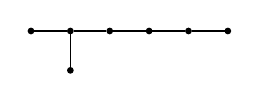
\begin{tikzpicture}[every node/.style={draw, circle, fill=black, minimum size=2pt, inner sep=0pt}]
\node[fill=black] (G1N2) at (5.50,5.00) {};
\node[fill=black] (G1N0) at (6.00,5.00) {};
\node[fill=black] (G1N1) at (6.50,5.00) {};
\node[fill=black] (G1N4) at (7.00,5.00) {};
\node[fill=black] (G1N5) at (7.50,5.00) {};
\node[fill=black] (G1N6) at (8.00,5.00) {};
\node[fill=black] (G1N3) at (6.00,4.50) {};
\draw (G1N0) -- (G1N1);
\draw (G1N0) -- (G1N2);
\draw (G1N0) -- (G1N3);
\draw (G1N1) -- (G1N4);
\draw (G1N4) -- (G1N5);
\draw (G1N5) -- (G1N6);
\end{tikzpicture}
\end{document}
